\documentclass{article}
\usepackage{tikz}
\usepackage{pgf-pie}
\usepackage{pgf-umlsd}
\begin{document}
random

\emph{\section{header 1}}
test words

\emph{\subsection{Test Case 7: Wide Tree Structure}}
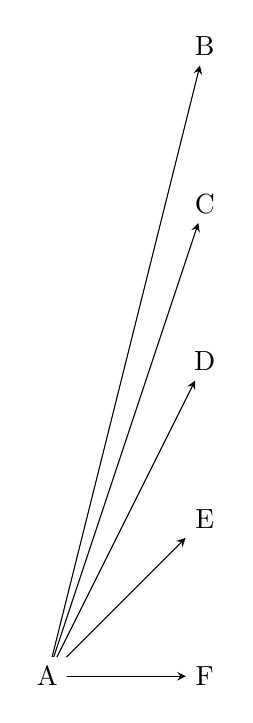
\begin{tikzpicture}[>=stealth]
\node (A) at (0, 2) {A};
\node (B) at (2, 10) {B};
\node (C) at (2, 8) {C};
\node (D) at (2, 6) {D};
\node (E) at (2, 4) {E};
\node (F) at (2, 2) {F};
\draw[->] (A) -- (B);
\draw[->] (A) -- (C);
\draw[->] (A) -- (D);
\draw[->] (A) -- (E);
\draw[->] (A) -- (F);
\end{tikzpicture}
more words same paragraph

test \emph{bold} test

test \textbf{bold} test test \emph{\textbf{bold}} test test _\textbf{bold} test

test no match *ag

test \emph{bold 3}

\emph{bold 4} test

\emph{\textbf{test }}what *

$1 + 1 = 2$

\emph{bold 2}

\textbackslash{}_bold\textbackslash{}*

\texttt{random code}\texttt{} wetwt

\href{www.test.com}{link}

test \emph{bold} \href{e.com}{link} tet

\begin{figure}[h]\centering\includegraphics{image.png}\caption{caption}\end{figure}

\begin{verbatim}
test
tickles

foo
\end{verbatim}
\end{document}
